\documentclass{article}
\usepackage{amsmath}
\usepackage{amsfonts}
\usepackage{amssymb}
\usepackage{mathtools}
\usepackage{tcolorbox}
\usepackage[inline]{enumitem}
\usepackage[a4paper,margin=1in]{geometry}
\usepackage[normalem]{ulem}
\usepackage{graphicx}
\usepackage{tasks}
\settasks{label=(\alph*), label-offset=0.4em, label-width=1.5em}

\usepackage{fancyhdr}
\fancyhf{}
\setlength{\headheight}{36pt}
\renewcommand{\headrulewidth}{0pt}
\thispagestyle{fancy}
\lhead{Calculus Exercise}
\chead{Week 14 (8.1, 8.2, 9.1, 9.3)}
\rhead{\underline{ID:\hspace{7.4em}} \\ \vspace{0.2cm} \uline{Name:\hspace{6em}}}
\cfoot{\thepage}

\begin{document}
\begin{enumerate}
\item[8.1.39]
    Find the length of the astroid.
    \begin{center}
        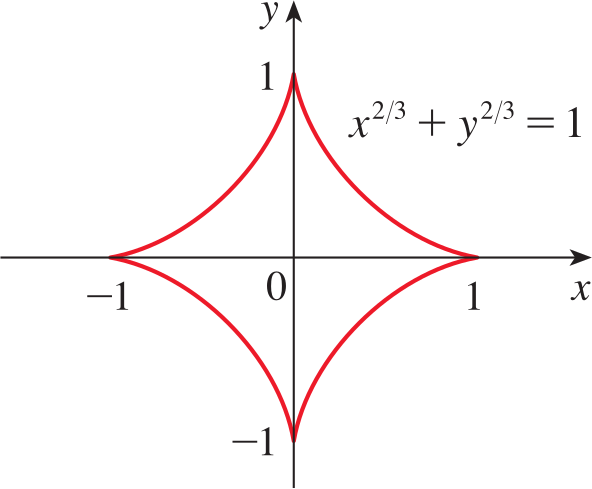
\includegraphics[height=4cm]{./png/8.1.39.png}
    \end{center}

\vspace{6cm}

\item[8.1.40]
    \begin{enumerate}
        \item Sketch the curve $y^{3} = x^{2}$.
        \item Use the two types of arc length formula
            \[
                \int_{a}^{b} \sqrt{1 + \left(\frac{dy}{dx}\right)^{2}} dx,\
                \int_{c}^{d} \sqrt{1 + \left(\frac{dx}{dy}\right)^{2}} dy
            \]
            to set up two integrals for the arc length from $(0, 0)$
            to $(1, 1)$. Observe that one of these is an improper integral and
            evaluate both of them.
        \item Find the length of the arc of this curve from $(-1, 1)$
            to $(8, 4)$.
    \end{enumerate}

\newpage

\item[8.1.43]
    Find the arc length function for the curve
    $y = \sin^{-1}x + \sqrt{1-x^{2}}$ with starting point $(0, 1)$.


\vspace{6cm}

\item[8.1.46]
    A steady wind blows a kite due west. The kite's height above ground from
    horizontal position $x=0$ to $x=80$ ft is given by $y=150 - \frac{1}{40}(x-50)^{2}$.
    Find the distance traveled by the kite.

\vspace{6cm}

\item[8.2.28]
    Find the exact area of the surface obtained by rotating the curve
    $y=\sqrt{x^{2}+1},\ 0 \leqslant x \leqslant 3$, about the $x$-axis.

\newpage

\item[8.2.33]
    \textbf{Gabriel's Horn} The surface formed by rotating the curve
    $y=\frac{1}{x}, x \geqslant 1$, about the $x$-axis is known as
    \textit{Gabriel's horn}. Show that the surface area is infinite (although the
    enclosed volume is finite.)

    \begin{center}
        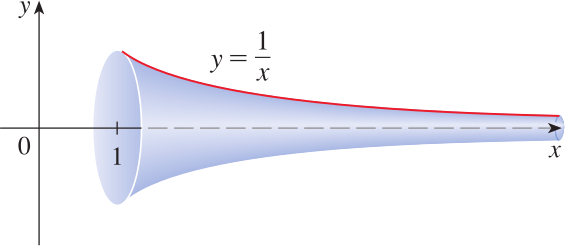
\includegraphics[height=3cm]{./png/8.2.33.png}
    \end{center}

\vspace{7cm}

\item[8.2.37]
    \begin{enumerate}
        \item The ellipse
            \[
                \frac{x^{2}}{a^{2}} + \frac{y^{2}}{b^{2}} = 1,\ a > b
            \]
            is rotated about the $x$-axis to form a surface called an \textit{ellipsoid},
            or \textit{prolate spheroid}. Find the surface area of this ellipsoid.
        \item If the ellipse in part (a) is rotated about its minor axis
            (the $y$-axis), the resulting ellipsoid is called an
            \textit{oblate spheroid}. Find the surface area of this ellipsoid.
    \end{enumerate}

\newpage


\item[8.2.42]
    \textbf{Zone of a Sphere} A \textit{zone of a sphere} is the portion of the
    sphere that lies between two parallel planes.

    Show that the surface area of a zone of a sphere is $S = 2\pi R h$,
    where $R$ is the radius of the sphere and $h$ is the distance between
    the planes. (Notice that $S$ depends only on the distance between the planes
    and not on their location, provided that both planes intersect the sphere.)

\vspace{5cm}

\item[9.1.19]
    \begin{enumerate}
        \item What can you say about a solution of the equation $y'=-y^{2}$ just
            by looking at the differential equation?
        \item Verify that all members of the family $y=\frac{1}{x+C}$
            are solutions of the equation in part (a).
        \item Can you think of a solution of the differential equation $y'=-y^{2}$
            that is not a member of the family in part (b)?
        \item Find a solution of the initial-value problem
            $y' = -y^{2},\ y(0) = 0.5$.
    \end{enumerate}

\vspace{5cm}

\item[9.1.21]
    A population is modeled by the differential equation
    \[
        \frac{dP}{dt} = 1.2P \left( 1 - \frac{P}{4200} \right)
    \]
    \begin{enumerate}
        \item For what values of $P$ is the population increasing?
        \item For what values of $P$ is the population decreasing?
        \item What are the equilibrium solutions?
    \end{enumerate}

\newpage

\item[9.1.25]
    Match the differential equations with the solution graphs labeled I-IV.
    Give reasons for your choices.
    (a) $y'=1+x^{2}+y^{2}$
    \hspace{0.5cm}
    (b) $y'=xe^{-x^{2}-y^{2}}$
    \hspace{0.5cm}
    (c) $y'=\frac{1}{1+e^{x^{2}+y^{2}}}$
    \hspace{0.5cm}
    (d) $y'= \sin (xy) \cos (xy)  $

    \begin{center}
        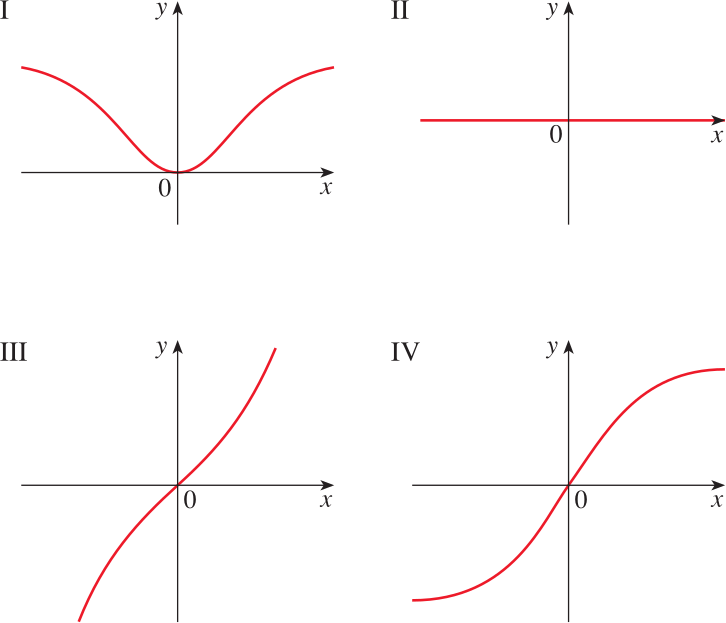
\includegraphics[height=6cm]{./png/9.1.25.png}
    \end{center}

\vspace{5cm}

\item[9.1.29]
    Differential equations have been used extensively in the study of drug dissolution
    for patients given oral medications. One such equation is the Weibull equation
    for the concentration $c(t)$ of the drug:
    \[
        \frac{dc}{dt} = \frac{k}{t^{b}}(c_{s}-c)
    \]
    where $k$ and $c_{s}$ are positive constants and $0 < b < 1$.

    Verify that
    \[
        c(t) = c_{s}(1-\exp(-\alpha t^{1-b}))
    \]
    is a solution of the Weibull equation for $t > 0$, where $\alpha = \frac{k}{1-b}$.
    What dose the differential equation say about how drug dissolution occurs?

\newpage

\item[9.3.42]
    In elementary chemical reaction, single molecules of two reactants A and B from
    a molecule of the product C: A + B $ \longrightarrow $ C. The law of mass action
    states that the rate of reaction is proportional to the product of the concentrations
    of A and B:
    \[
        \frac{d[\text{C}]}{dt} = k [\text{A}][\text{B}]
    \]

    Thus if the initial concentrations are $[\text{A}] = a$ moles/L
    and $[\text{B}] = b$ moles/L and we write $x = [\text{C}]$, then we have
    \[
        \frac{dx}{dt} = k(a-x)(b-x)
    \]
    \begin{enumerate}
        \item Assuming that $a \neq b$, find $x$ as a function of $t$.
            Use the fact that the initial concentration of C is 0.
        \item Find $x(t)$ assuming that $a=b$. How does this expression for $x(t)$
            simplify if it is known that [C]$=\frac{a}{2}$ after 20 seconds?
    \end{enumerate}

\vspace{6cm}

\item[9.3.44]
    A sphere with radius 1 m has temperature $15^{\circ}$C. It lies inside a concentric
    sphere with radius 2 m and temperature $25^{\circ}$C. The temperature $T(r)$ at
    a distance $r$ from the common center of the spheres satisfies the differential
    equation
    \[
        \frac{d^{2}T}{dr^{2}} + \frac{2}{r}\frac{dT}{dr} = 0
    \]
    If we let $S = \frac{dT}{dr}$, then $S$ satisfies a first-order differential
    equation. Solve it to find an expression for the temperature $T(r)$ between the
    spheres.

\newpage

\item[9.3.48]
    The air in a room with volume $180$ m$^{3}$ contains 0.15\% carbon dioxide initially.
    Fresher air with only 0.05\% carbon dioxide flows into the room at a rate of
    2 m$^{3}$/min and the mixed air flows out at the same rate. Find the percentage
    of carbon dioxide in the room as a function of time. What happens in the long run?

\vspace{6cm}

\item[9.3.54]
    A model for tumor growth is given by the Gompertz equation
    \[
        \frac{dV}{dt} = a (\ln b - \ln V) V
    \]
    where $a$ and $b$ are positive constants and $V$ is the volume of the tumor measured
    in mm$^{3}$.
    \begin{enumerate}
        \item Find a family of solutions for tumor volumes as a function of time.
        \item Find the solution that has an initial tumor volume of
            $V(0) = 1 \text{mm}^{3}$.
    \end{enumerate}

\end{enumerate}
\end{document}
